%Chapter 2

\renewcommand{\thechapter}{2}

\chapter{A Geo-Distributed System Architecture}
\label{ch:architecture}

% Goals for this chapter:
%   1. Present a case that geo-replicated systems are more common
%   2. Present the challenges for a geo-replicated system
%   3. Outline our proposed architecture
%   4. Outline our proposed apps: distributed log, kv store, file system

% At the end of this chapter the reader should believe that planetary-scale  data systems are necessary and that existing solutions don't meet current requirements exactly.

% The primary purpose of this chapter is to show that our core component, hierarchical consensus is the center of any geo-replicated system.

The advent of cloud computing has accelerated both commercial and academic interest in distributed systems connected via wide area networks and the Internet.
Cloud computing exists because large Internet companies, which had deployed extremely large data centers around the world to meet global user demand for their services, created extra capacity that could be leased to tenants on-demand.
The global nature of cloud providers means that there is an opportunity for more common usage of geographically replicated data systems besides the specialized systems they developed for internal use.
Though these systems have been made available to customers as provisioned services, they suffer from application-specific data models too narrow to solve general problems.

The specialization of the current generation of distributed systems is designed to optimize their behavior when deployed within a pristine data center context.
This environment, with strong facility support and backbone communications, allows design choices that optimistically assume that repairs will be made quickly and that redundancy need only protect from few failures at a time~\cite{bermbach_eventual_2011,wada_data_2011,node_failure,jhawar_fault_2013}.
This has led to a general architecture for geo-replication that provisions consistency requirements across transactions, individual objects, and within blocks stored on disk, often leading to multiple, independent consistency models within the same system.
This design leads to confusion about where data is stored and what guarantees can be made about each access.

Instead, a single, global consistency model is required to correctly reason about a single, global system's behavior.
The central thesis of this dissertation is that this can only be achieved with a globally-distributed consensus protocol.

Consistency depends on the network environment and in highly curated data centers, systems are built using localized consensus~\cite{bolosky_paxos_2011}.
Outside the data center, however, single process failures show the impossibility of distributed consensus~\cite{fischer_impossibility_1985}.
Therefore our approach is a continuous, flexible consistency model with geographic consensus at its core and a federated approach at its edge.
The result is a single, understandable consistency model that leads to an architecture capable of supporting global systems both inside and outside of the data center.

In this chapter, we will describe the details of our proposed architecture for a planet-wide distributed data store.
To motivate our architectural decisions, we first describe the motivations and challenges for the design of such a system.
We motivate our work in two parts.
First, we argue that there is a new software deployment paradigm that requires geographic replication.
Second, we argue that existing geo-replicated data stores are not general enough to meet the needs of that paradigm.
We follow these motivations with the challenges of geo-replication described as requirements, which we will then use to present an overview of our system architecture.

\section{Challenges and Motivations}
\label{ch02_challenges_and_motivations}

Many of the world's most influential companies grew from the ashes of the dot-com bubble of the 1990s, which paid for an infrastructure of fiber-optic cables, giant server farms, and research into mobile wireless networks~\cite{casey_blockchain_2018}.
As these companies filled market voids in eCommerce, search, and social networking, they created new database technologies to leverage the potential of underused computational resources and low latency/high bandwidth networks that connected them, eschewing more mature systems that were developed with resource scarcity in mind~\cite{stonebraker_what_2005,stonebraker_mapreduce_2010}.
What followed was the rise and fall of NoSQL data systems, a microcosm of the proceeding era of database research and development~\cite{mohan_history_2013}.

Although there are many facets to the story of NoSQL, what concerns us most is the use of NoSQL to create geographically distributed systems, as these systems paved the way to the large-scale storage systems in use today.
The commercial and open source interest in geo-replicated systems both for big data analysis and Web application development has led to the development of many database and file systems.
These systems share common traits, allowing us to describe a general architecture for distributed systems.
More importantly, the prevalence of such systems has led to a new application development paradigm: modern software must be designed as a global service.

\subsection{A New Application Development Paradigm}
\label{ch02_new_software_paradigm}

The launch of the augmented reality game Pokémon GO in the United States was an unmitigated disaster~\cite{kain_pokemon_2016}.
Due to extremely overloaded servers from the release's extreme popularity, users could not download the game, login, create avatars, or find augmented reality artifacts in their locales.
The company behind the platform, Niantic, scrambled quickly, diverting engineering resources away from their feature roadmap toward improving infrastructure reliability.
The game world was hosted by a suite of Google Cloud services, primarily backed by the Cloud Datastore~\cite{cloud_datastore}, a geographically distributed NoSQL database.
Scaling the application to millions of users therefore involved provisioning extra capacity to the database by increasing the number of shards as well as improving load balancing and autoscaling of application logic run in Kubernetes~\cite{Kubernetes} containers.

Niantic's quick recovery is often hailed as a success story for cloud services and has provided a model for elastic, on demand expansion of computational resources.
A deeper examination, however, shows that Google's global high speed network was at the heart of ensuring that service stayed stable as it expanded ~\cite{stone_bringing_2016}, and that the same network made it possible for the game to immediately become available to audiences around the world.
The original launch of the game was in 5 countries -- Australia, New Zealand, the United States, the United Kingdom, and Germany.
The success of the game meant worldwide demand, and it was subsequently expanded to over 200 countries starting with Japan~\cite{yamazaki_developer_2016}.
Unlike previous games that were restricted with region locks~\cite{region_locking}, Pokémon GO was a truly international phenomenon and Niantic was determined to allow international interactions in the game's feature set, interaction which relies on Google's unified international architecture and globally distributed databases.

Stories such Niantic's deployment are increasingly becoming common and medium to large applications now \emph{require developers to quickly reason about how data is distributed in the wide area, different political regions, and replicated for use around the world}.

It is not difficult to find many examples of companies and applications, from large to small, that have international audiences and global deployments which highlight the new challenges of software development.
Dropbox has users in over 180 countries and is supported in 20 languages, maintaining offices in 12 locations from Herzliya to Sydney \cite{dropbox}.
Slack serves 9 million weekly active users around the world and has 8 offices around the world, prioritizing North America, Europe, and Pacific regions \cite{slack}.
WeWork provides co-working space in 250+ international applications and uses an app to manage global access and membership \cite{wework_global_access}.
Tile has sold 15 million of its RFID trackers worldwide and locates 3 million unique items a day in 230 countries \cite{tile}.
Trello, a project management tool, has been translated into 20 languages and has 250 million world-wide users in every country except Tuvalu; their international rollout focused on marketing and localization \cite{trello}.
Runkeeper~\cite{runkeeper} and DarkSky~\cite{darksky} are iOS and Android apps that have millions of global users and struggled to make their services available in other countries, but benefitted from international app stores.
Signal and Telegraph, both encrypted messaging apps, have grown primarily in countries at the top of Transparency International's Corruption Perception Index~\cite{signal}.

The new application development paradigm, even for small applications, is to build with the thought that your application will soon be scaling across the globe.
None of the applications described above necessarily have geography-based requirements in the same way that an augmented reality or airline reservations application might, just a large number of users who regularly use the app from a variety of geographic locations.
Web developers are increasingly discussing and using container based approaches both for development and small-scale production.
Web frameworks have built in localization tools that are employed by default.
Services are deployed on autoscaling cloud platforms from the start.

To address this paradigm shift, cloud service providers have expanded their offerings to include use of their distributed data stores to application developers, as in the case of Niantic.
This presents two problems, however.
First, those systems were designed for the huge applications of the Internet companies themselves, not for the general needs of a large audience of developers.
Second, cloud providers organized their services around geographically distinct regions, allowing their tenants the choice to deploy their applications in one or more regions.
As a result, tenants naturally choose cloud regions based on the locations of their users and treat regions as independent deployments from both a software and billing perspective.
Even though there may be some cross-region backup to prevent catastrophic failures, region-specificity usually means that services are deployed piecemeal and partitioned.

Region-based organization of cloud services has ensured that users are able to minimize latencies and provide applications to areas of interest, but applications have increasingly become more global.
The possibility of region-agnostic deployment is tantalizing, particularly as larger applications spend a non-trivial amount of administration time determining where writes to objects are going to optimize their systems.
Consistent updates across regions are not generally considered as a possibility because in-house cloud services used data models that avoided large latencies wherever possible.
Moreover, as we will see in the next section, the design of provisioned cloud databases have made it difficult to reason about consistent behavior.
Not only is there a need for strong consistency semantics, data-location awareness, and geo-replication in distributed data storage systems, there is also the need for a familiar and standardized storage API.

\subsection{Building Geo-Replicated Services}
\label{ch02_systems_background}

The growth of database systems distributed across the wide-area started with large Internet companies like Yahoo~\cite{pnuts}, Google~\cite{bigtable}, and Amazon~\cite{dynamo} but quickly led to academic investigations.
One reason that the commercial systems enjoyed this academic attention was that at the time, the unique scale of their usage validated the motivation behind their architecture.
However their success has meant that these types of scales are no longer limited to huge software systems.
The development of geo-replicated services has therefore undergone several phase shifts, and has led to a general framework that underlies most current systems.
In this section we outline these phases and describe the general framework with a blueprint for designing large-scale distributed systems (see Figure~\ref{fig:ch02_distributed_architecture}), which we then use to motivate our system architecture.

The first shift was the creation of highly available, sharded systems intended to meet the demand of increasing numbers of clients.
Commercially, these types of systems include Dynamo~\cite{dynamo} and BigTable~\cite{bigtable}, which in turn spawned open source and academic derivatives such as Cassandra~\cite{cassandra} and HBase~\cite{hbase}.
Although these systems did support many concurrent accesses, they achieved their availability by relaxing consistency, which many applications found to be intolerable.
The second shift was a return to stronger consistency, even at the cost of decreased performance or expensive engineering solutions.
Again, commercial systems led the way with Megastore~\cite{megastore} and Spanner~\cite{spanner} along with academic solutions such as MDCC~\cite{mdcc} and Calvin~\cite{calvindb,calvinfs}.
Part of this realignment was a reconsideration of the base assumptions that drove the NoSQL movement as expressed in the CAP theorem~\cite{cap,pushing_cap}.
The new thinking is that the lines between availability, partition tolerance, and consistency may not be as strictly drawn as previously theorized~\cite{hat,consistency_tradeoffs,cap_rules_change}.
This has led to a final shift, the return of SQL, as the lessons learned during the first two phases are applied to more traditional systems.
As before, both commercial systems, such as Aurora~\cite{aurora} and Azure SQL~\cite{azure_sql_database}, and open source systems such as Vitess~\cite{vitess} and CockroachDB~\cite{cockroachdb} are playing an important role in framing the conversation about consistency in this phase.

% This brief and limited description of the history of NoSQL distributed systems serves to set the tone for two primary points. First, designing distributed systems to support a large number of users across large geographies entails a number of challenges and trade-offs due to physical limitations that no single architecture has been able to fully cover. Second, there exists commercial and practical motivations to build such systems and these motivations have been the impulse toward academic research. With this backdrop in mind, we explore in this chapter the question of whether a planetary-scale data system is really necessary, and the challenges that we face when designing such systems.

These systems have defined several strategies from relaxed consistency to interval time that are essential to understanding geo-replicated services.
The first and primary strategy, however, is to shard data into independent groups of semi-related objects.
A shard can be specifically defined either as buckets of objects, tablets of contiguous rows, or in the most extreme cases, individual objects.

Sharding allow extremely massive databases and file systems to be broken down into smaller, related pieces that are more easily managed in a distributed context.
Sharding allows concurrent access to objects without synchronization.
If a shard is defined within a specific region, then it is easy to prioritize local accesses and coordination with that region.
Sharding also provides a data model for underlying redundant storage.
If a tablet can be written to a specific page on disk, that page can also be replicated to more easily colocate replicas with data.
If multiple shards need to be accessed simultaneously in a transaction, then
only the shards involved in the transaction need be coordinated, while all other shards can remain independent.

The unit of coordination is therefore at the shard level.
The namespace of the system must be allocated to individual components of the system, which must be globally available, and requires coordination to move part of the namespace from one region to another.
Accesses to data on disk for individual objects must also be allowed to happen in a fault-tolerant manner, which requires coordination between several replicas to guarantee no data loss.
Finally, transactions that require access to multiple objects must be coordinated to ensure atomic guarantees.
To support all of these features in a system, a multi-process architecture of independent components for geo-replication is generally deployed, as shown in Figure~\ref{fig:ch02_distributed_architecture}.

\begin{figure}
    \begin{center}
        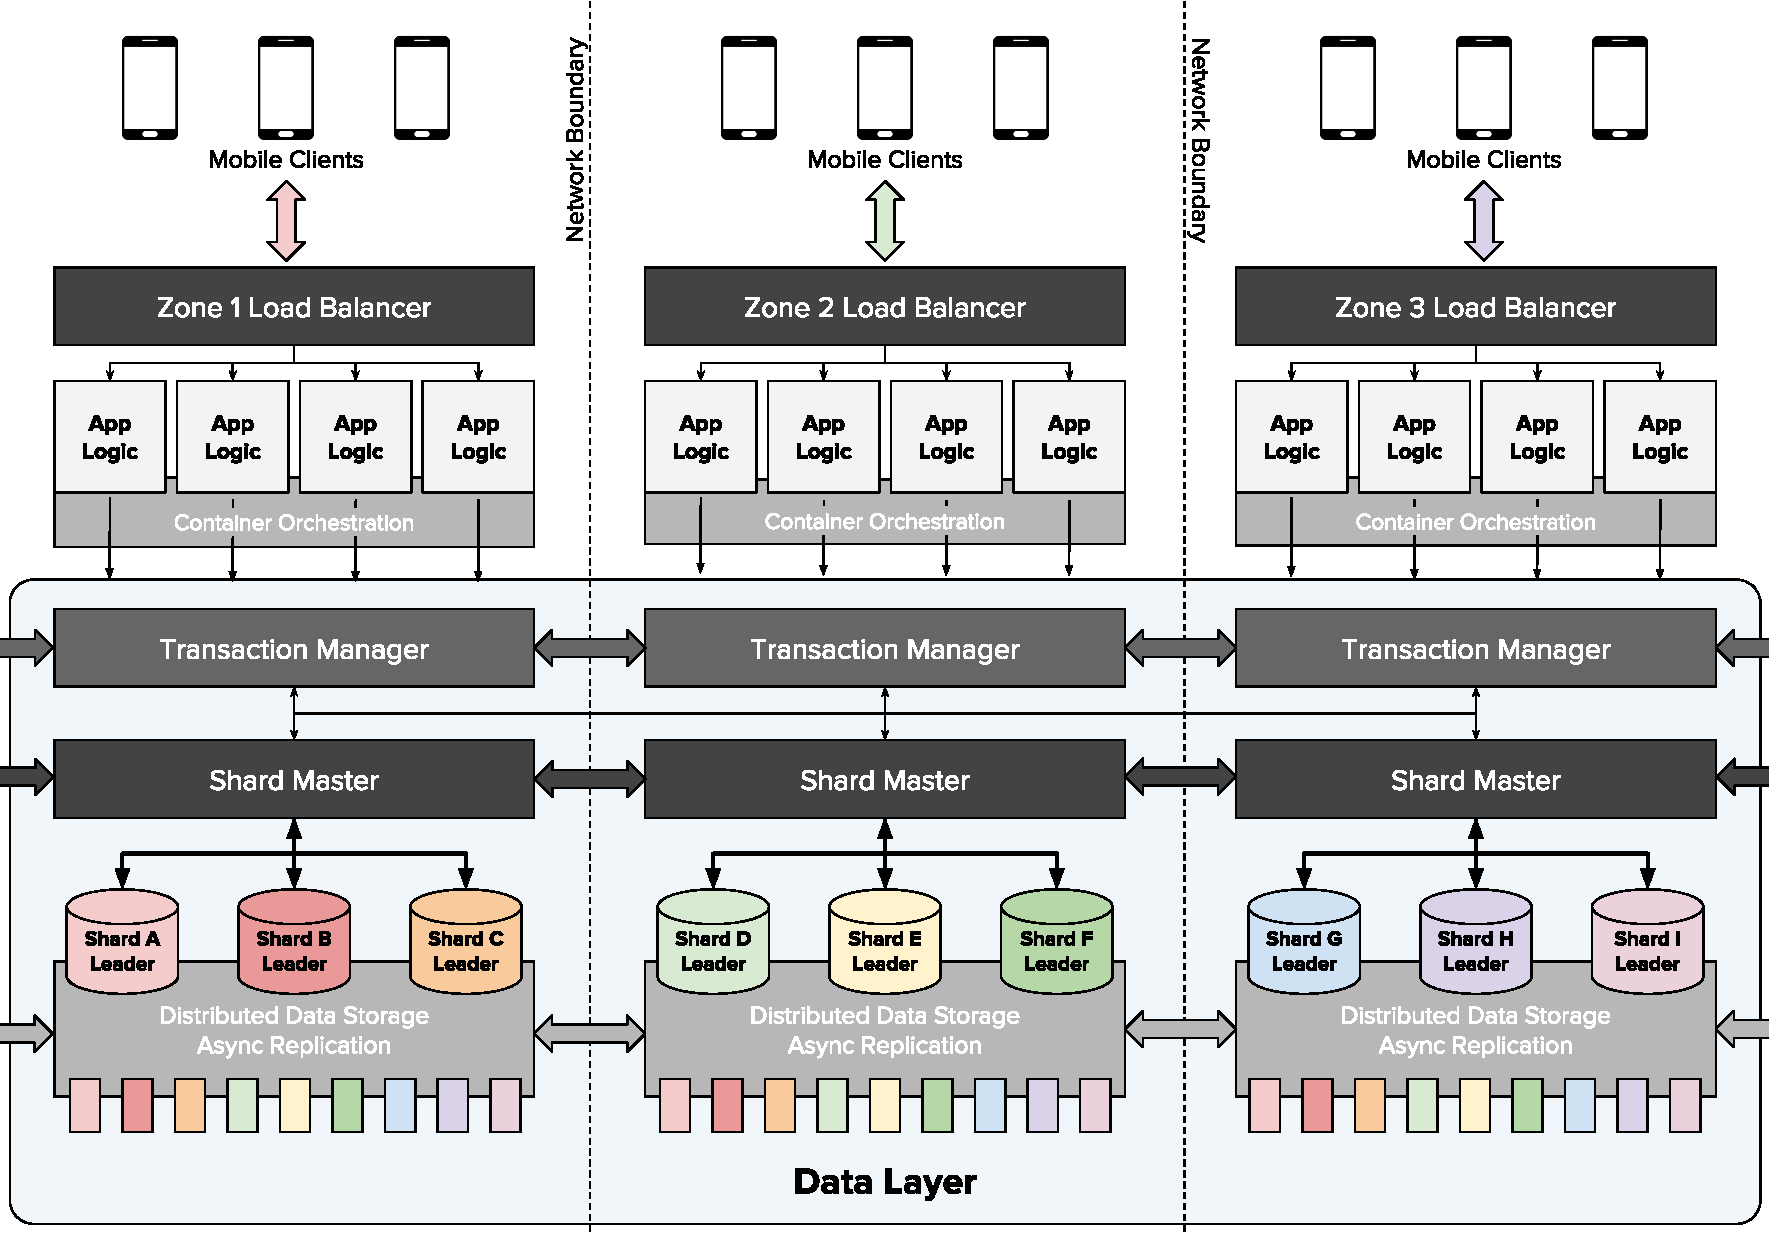
\includegraphics[width=5in]{figures/ch02_distributed_architecture.pdf}
    \end{center}
    \renewcommand{\baselinestretch}{1}
    \small\normalsize

    \begin{quote}
        \caption[A Generalized Geo-Distributed System Architecture]{A generalized architecture of a geographically distributed application using a basic sharding strategy. The namespace of the database is coordinated by shard masters, which point to quorums of replicas who replicate data over multiple disks. Accesses to multiple objects are coordinated via transaction managers.}
        \label{fig:ch02_distributed_architecture}
    \end{quote}
\end{figure}
\renewcommand{\baselinestretch}{2}
\small\normalsize

Clients access geographically-replicated data systems either by making geographic based requests via domain name (e.g. requesting a \texttt{.ca} addressed service vs. a \texttt{.fr} address) or by using IP and ping based network location~\cite{geoping}.
Multiple, concurrent requests are load-balanced to container based compute nodes that hold application logic, elastically scaled to meet changing demand~\cite{load_balancing}.
Though this aspect of distributed applications is outside the scope of a geo-replicated data store, the increased frequency of accesses across multiple regions increases the likelihood of collisions -- concurrent access by multiple clients to the same object(s), which leads to the consistency concerns of this dissertation.

The data layer follows the application logic layer and is the layer that must coordinate accesses from many simultaneous geographies.
If the data layer supports transactions~\cite{hat,calvindb,calvinfs,cockroachdb,vitess,aurora} then the top level of coordination is the transaction manager, which is responsible for identifying the shards that manage the objects and correctly committing or rolling back the transaction.
Other systems support snapshot isolation for read-transactions~\cite{spanner,megastore}, ensuring that all reads for a specified time window are consistent.

If the data layer does not support transactions or if only a single object is being accessed, then the system must coordinate with the shard master, a process that allocates the namespace to the replicas that manage those objects.
Some systems use the data-model directly, using key-space addressing to determine the locality of objects~\cite{bigtable,spanner}, others use consistent hashing~\cite{chord,scatter} to balance objects around a hash ring, coordinating the insertion and removal of name management servers.
However, if the preservation of data locale and the ability to move objects between regions is required, then a synchronized lookup table must be used.
The most popular mechanism to achieve namespace synchronization is to use a lock service such as Chubby~\cite{chubby} or etcd~\cite{etcd_raft} to hand out leases for which an replica is expected to manage accesses.

Once the replica that manages the shard is discovered, the actual access must occur.
There are several mechanisms for this that use quorums of replicas to make decisions.
Weak consistency models of access use overlapping read and write quorums of varying sizes along with eventual replication of the data~\cite{dynamo}.
Strong consistency models of access use Paxos~\cite{paxos} as the basis for high performance data storage~\cite{bolosky_paxos_2011,lampson_how_1996} -- consensus will be discussed in detail in the next section.
To further increase write throughput, accesses append commands to a distributed log that are applied asynchronously to the underlying data store, so long as the command is committed to the log, it is guaranteed to be written to storage~\cite{logbase,logfs,log_memory}.

Finally, data must be written to stable storage, usually on clusters of disks that are also distributed so as to prevent data loss in the likely event that a disk fails.
Many geo-replicated data systems also use a distributed file system for underlying storage.
BigTable stores its data on GFS~\cite{gfs}, f4~\cite{f4} on top of HDFS~\cite{hdfs}, an open source implementation of GFS, and Spanner stores its data on Colossus~\cite{colossus}, the next generation of GFS.
Other distributed databases such as BTrDB~\cite{btrdb} use the Ceph~\cite{ceph} file system for data replication and because of requirements for location-fault tolerance, it is becoming increasingly rare that hardware based schemes such as RAID~\cite{raid} are used to ensure data durability.

\begin{figure}
    \begin{center}
        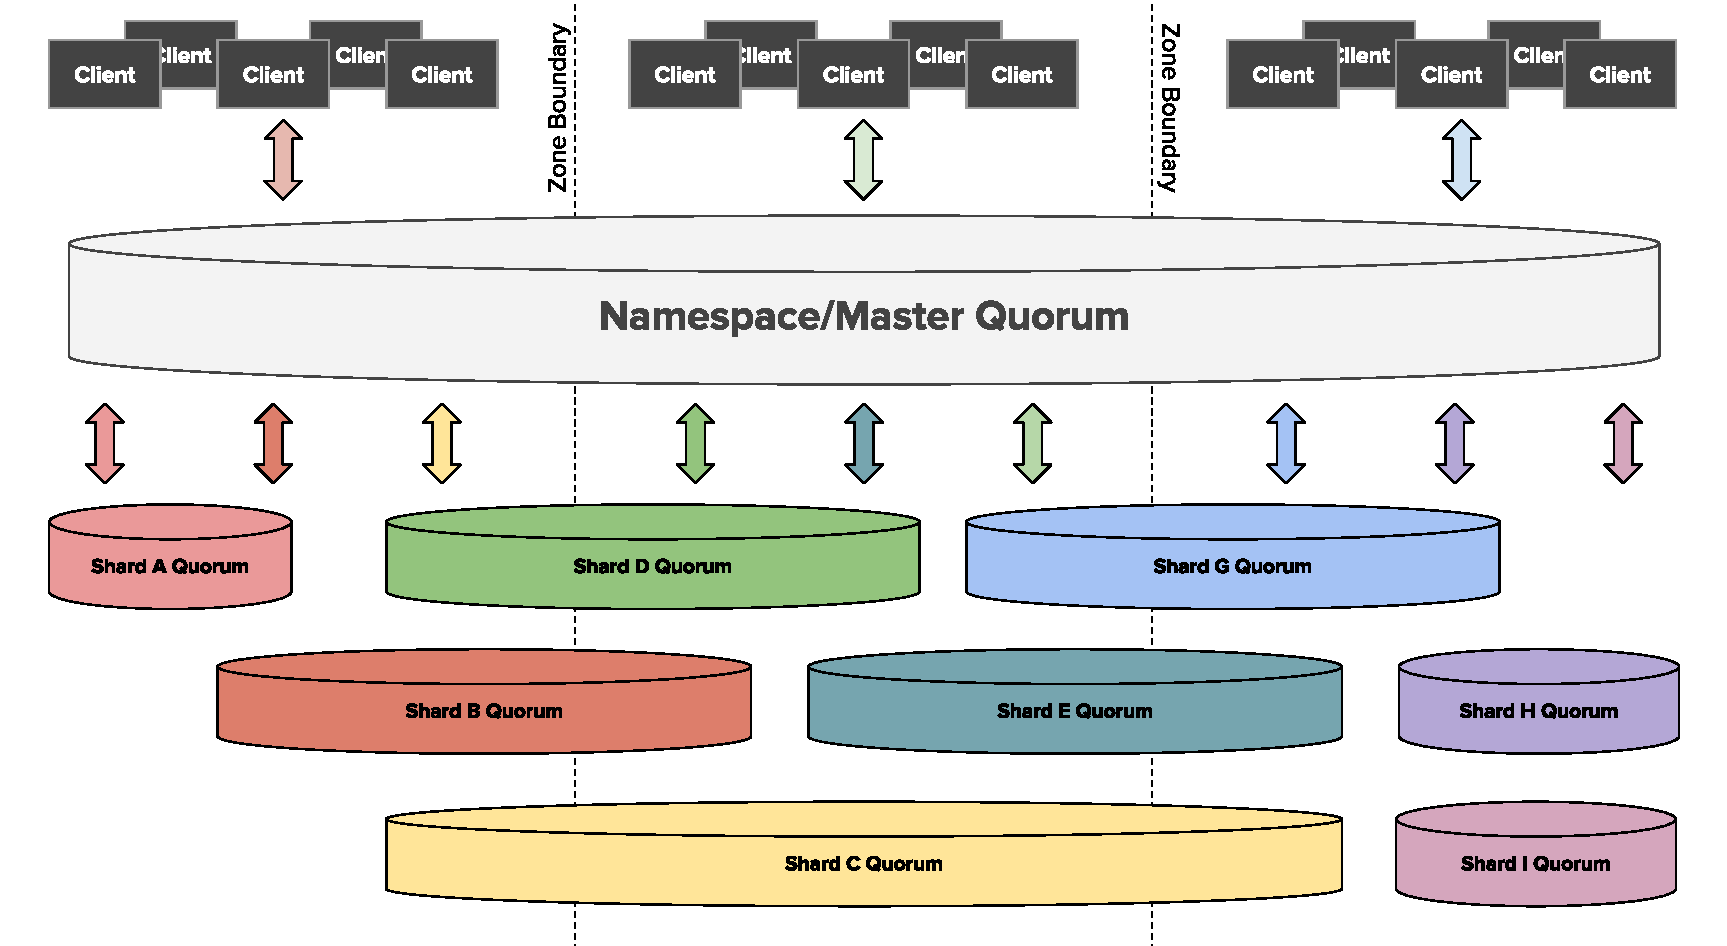
\includegraphics[width=5in]{figures/ch02_simplified_distributed_consensus_alt.pdf}
    \end{center}
    \renewcommand{\baselinestretch}{1}
    \small\normalsize

    \begin{quote}
        \caption[A Simplified Geo-Distributed Consensus Blueprint]{Figure~\ref{fig:ch02_distributed_architecture} can be simplified to a single consensus architecture with a top-level consensus quorum making namespace decisions and directing requests to per-object quorums that are replicated within a single data center or across regions or zones.}
        \label{fig:ch02_simplified_distributed_consensus}
    \end{quote}
\end{figure}
\renewcommand{\baselinestretch}{2}
\small\normalsize

The description above and Figure~\ref{fig:ch02_distributed_architecture} are a useful blueprint for designing large scale geo-replicated systems and generalizes many of the themes and attributes of a wide variety of systems.
The problem with this blueprint is that it imposes a multi-process system architecture; replicas are coordinated by master processes and lock services, and then store data on distributed file systems, yet more processes with independent coordination.
Multiprocess systems then must be further coordinated so that the health and status of each process must be known, leading to the use of monitoring and management tools like Ambari~\cite{ambari} and Zookeeper~\cite{zookeeper}.
With so many layers of coordination, it becomes impossible to reason about consistency and data locality, and such systems become very difficult to deploy without excellent systems administration.

We propose that the complexity of this blueprint can be simplified instead to a multiple consensus process model as shown in Figure~\ref{fig:ch02_simplified_distributed_consensus}.
This model does not eliminate the components described in the blueprint, but rather consolidates them into two primary coordination activities: coordinating the namespace and coordinating accesses to and storage of objects.
In this model, a single geo-replicated quorum manages the global namespace -- the primary master process.
Multiple independent subquorums manage accesses to individual objects, replicated solely within a single datacenter, replicated across zones, or replicated across the wide area.

This simplification makes it clear that the core of a fault-tolerant, geo-replicated distributed system is effective distributed consensus that can scale to multiple replicas across many regions and can survive failures that may occur in wide area systems.
In the next section, we will build upon this idea and describe an overview of our proposed architecture along with consistency and failure requirements.

\section{System Architecture}
\label{ch02_architecture}

We propose a consistency-centric approach to designing distributed data stores, centered on geographically distributed consensus.
Modern software is developed with international audiences in mind from the outset and requires data services that span oceans, continents, and political regions.
Existing large-scale database and file systems were purpose built for gigantic applications created by large Internet companies and include specializations for data-center level computer engineering.
These specializations resulted in complex coordination divided between levels to manage transactions, namespace allocation, accesses, and storage.
To ensure a wider audience of software developers can correctly reason about consistency across the wide area a single, global consistency model is required.

Geographically distributed consensus is not sufficient, however, as system environments are migrating outside of the data center.
The next generation of geo-distributed systems will require edge replicas to support high-throughput writes from sensor networks deployed on the energy grid, traffic coordination networks, and the Internet of Things.
A consistency-centric approach requires therefore that both strong consistency and high availability replicas are federated into a single model of consistency.
Our architecture therefore leverages a hierarchical consensus model to provide strong consistency across regions, centralized by data center along with a federated consistency model for a fog of edge devices surrounding data centers to support heterogenous network environments.

In this section we will first describe a consistency model that informs our architectural decisions.
Next, we will describe the requirements for distributed systems that our architecture addresses.
Finally, we will provide an overview of our planet-scale architecture that serves as the foundation for this dissertation.

\subsection{Consistency and Consensus}
\label{ch02_consistency}

Our consistency model is a \textit{data-centric} model, as opposed to a \textit{client-centric} model~\cite{bermbach_consistency_2013}.
Client-centric models view the system as a black box and consistency is described as guarantees made to processes or applications that interact with the system such as ``read your writes'' or ``write follows read''~\cite{eventual_consistency}.
Data-centric consistency on the other hand is concerned about the ordering of operations applied to a replica and generally considers the problem of how those operations relate to each other in a per-replica, append-only log.

Data-centric consistency can be reasoned about by considering a log-based model of consistency.
Replicas in a distributed system can be viewed as independent state machines that apply commands in response to client requests or messages from other replicas~\cite{state_machine_approach}.
Each command is appended to a log that records a time-ordered sequence of operations such that from the same starting state, every time the log is replayed the replica will reach the same ending state.
Two replicas are locally consistent (consistent with each other) if their logs are able to bring them to identical states.
Global consistency requires all replicas logs express a single, abstract ordering that brings the entire system to identical states.

Neither local nor global consistency requires replica logs to be identical, only that a log, when applied, leads to the same state.
Consistency guarantees can therefore be described by specifying how the logs of two replicas or all logs in a system are allowed to vary.
These variations can generally be described along two dimensions: staleness and ordering.

\begin{enumerate}
    \item \emph{Staleness} refers to how far behind the latest global state a local log is and can be expressed by the visibility latency of distributing a command to all replicas or simply by how many updates the log is behind by.
    \item \emph{Ordering} refers to how closely individual logs adhere to an global chronological ordering of commands. A strict ordering requires all logs or some prefix of the log to be identical, whereas weaker ordering allows some divergence in order updates applied to the log.
\end{enumerate}

Most data-centric consistency models refer to the strictness of ordering guarantees and the method by which updates are applied to the state of the replica~\cite{tanenbaum_distributed_2007}.
The least strict model, weak consistency (WC) makes no guarantees whatsoever about the relationship of local and remote writes and requires no coordination.
Eventual consistency (EC) is primarily concerned with the final state of all logs given some period of quiescence that allows the system to converge~\cite{anti_entropy}.
Though two logs may have an entirely different ordering of commands and not all commands may be present in all logs, EC guarantees that all replicas will achieve the same state, eventually.
Causal consistency (CC) ensures that a log is as up to date as all other logs with respect to a subset of dependencies~\cite{causal,causal_2}.
Sequential consistency (SC) is a strong consistency model that requires all replicas have the same exact log ordering on a per-object or multi-object basis, but does not make guarantees about staleness~\cite{sequential_consistency,sequential_consistency_2}.
Finally, linearizablity (LIN), the strongest form of consistency, requires that clients see a single, externalizable log no matter which part of the system they access~\cite{linearizability}.

Consensus algorithms~\cite{paxos,paxos_simple,paxos_practical,paxos_live,epaxos,fast_paxos,spaxos,multicoordinated_paxos,generalized_paxos,raft} are used to coordinate the logs of replicas to provide strong consistency in a distributed system.
Consensus requires two phases to ensure a command is correctly committed to a majority of replica logs.
The first phase, \emph{PREPARE}, allows a replica to nominate a slot in the log for a specific command.
If the majority of the replicas agree to allow the replica that slot, the second phase, \emph{ACCEPT}, allows a majority of replicas to agree that they have placed a specific command in specified log slot.
At the cost of multiple coordination messages per access, consensus guarantees that all replicas will always have identical logs.

Because enforcing log ordering requires increased coordination between replicas, there is a trade-off between ordering strictness and staleness that often defines the choice of consistency model used in a distributed system.
Coordination adds dependencies to accesses that introduces latency when responding to clients and total failure if part of the system is not available~\cite{fischer_impossibility_1985}.
Eventually consistent models reduce coordination and susceptibility to failure by creating relaxing quorum membership and using asynchronous synchronization.
By relaxing ordering strictness, the system is able to respond more quickly but the reduction in coordination causes staleness, which is the root of all observed inconsistencies in the system~\cite{probabilistically_bounded_staleness,quantifying_pbs}.
Staleness is entirely dependent on latency, therefore, in a data-center context, eventual consistency has been considered consistent enough.
In a geo-replicated context, however, the requirements for data systems change as the physical properties of networks become more apparent.

\subsection{Requirements for Data Systems}
\label{ch02_requirements}

We contend that \emph{consistency depends on the network environment}.
A network with instantaneous and perfectly reliable communications would never be inconsistent because all updates could be applied simultaneously with no latency.
Real world networks have to contend with physical systems and distances that create meaningful delays when coordinating messages.
Eventually consistent systems depend on the speed at which updates are disseminated through the network -- the slower the dissemination, the more likely that an inconsistency is observed.
Strong consistency systems implemented with consensus are provably correct but will fail to make progress as network conditions deteriorate.
In a geo-replicated system, consistency challenges are even greater because latencies are larger and outages more widespread.
Most proposed geo-replicated systems~\cite{redblue,hat,wren,walter,eiger,alvaro2013consistency} therefore attempt to find some balance of consistency models, trading off between the types of expected failures.
In this section we will briefly describe our expectations for network conditions and the requirements for our data system.

In large systems with thousands of replicas and millions of clients, failure is common and should be expected~\cite{node_failure}.
Disk failure is the most destructive form of failure in a system because it leads to permanent data loss and can only be managed through redundancy.
Replica failure either due to hardware failure or power loss, though temporary, reduces the total availability of the system.
Homogeneity in both disks and replicas can also lead to correlated failures, causing an extremely destructive cascading effect~\cite{f4}.

In addition to node failures, communication failure must also be resolved.
We assume a reliable network protocol that buffers messages and ensures delivery if a replica can be communicated with, messages are not dropped so long as the recipient is online.
We therefore treat network failures as partitions such that replicas cannot communicate with some subset of its peers.
In the case of either replica or network failure, once replicas can communicate and are back online, they must be able to gracefully rejoin the system.

In a geo-replicated context, large latencies are not primary issue, rather variability in expected latencies are.
Access patterns are typically location-dependent and correlated with respect to time (e.g. there are more accesses during daylight business hours).
There is a known physical limit to message traffic and with deterministic latency a network could be constructed to efficiently and correctly propagate data around the system.
Unfortunately, because both partitions and latency are variable, systems must be designed to be fully connected to all areas of the network.

In the face of failure, the primary requirements for a geo-replicated system are therefore durability, fault-tolerance, heterogeneity, and adaptability.
Durability normally considers three disk replication to ensure that 2 failures do not lead to data loss.
In a geo-replicated context, regions provide robustness in the case of catastrophic failures, e.g. a natural disaster that causes wide-spread power failures~\cite{cloud_deployments}.
Therefore durability and fault tolerance require not just disk replication but also zone and region replication.
Heterogeneity prevents both cascading, correlated failure, but also allows many different types of systems to participate in the network.
Finally adaptability allows the system to respond to changes in the network environment, both in terms of outages and user access patterns.
An adaptable system will also be able to dynamically add and remove nodes and scale with an increased number of regions.
With these requirements in mind, in the next section we describe our proposed architecture.

\subsection{A Planetary Scale Architecture}
\label{ch02_planetary_scale_architecture}

We envision a consistency-centric, planetary-scale distributed system as a two tier architecture shown in Figure~\ref{fig:ch02_global_architecture}.
The first tier resides inside of a data center environment and relies on high-speed backbone connections and high performance machines to implement geo-distributed consensus using the hierarchical consensus protocol, which we describe in Chapter~\ref{ch:hierarchical_consensus}.
The second tier is a highly-available network of edge replicas that disseminate updates in the wide area between data centers using a federated consistency model, which we will describe in Chapter~\ref{ch:federated_consistency}.
Such a large system requires machine learning mechanisms to monitor and adapt behavior according to changing network conditions, maximizing the consistency of the entire system, which we will describe in Chapter~\ref{ch:adaptive_consistency}.

\begin{figure}
    \begin{center}
        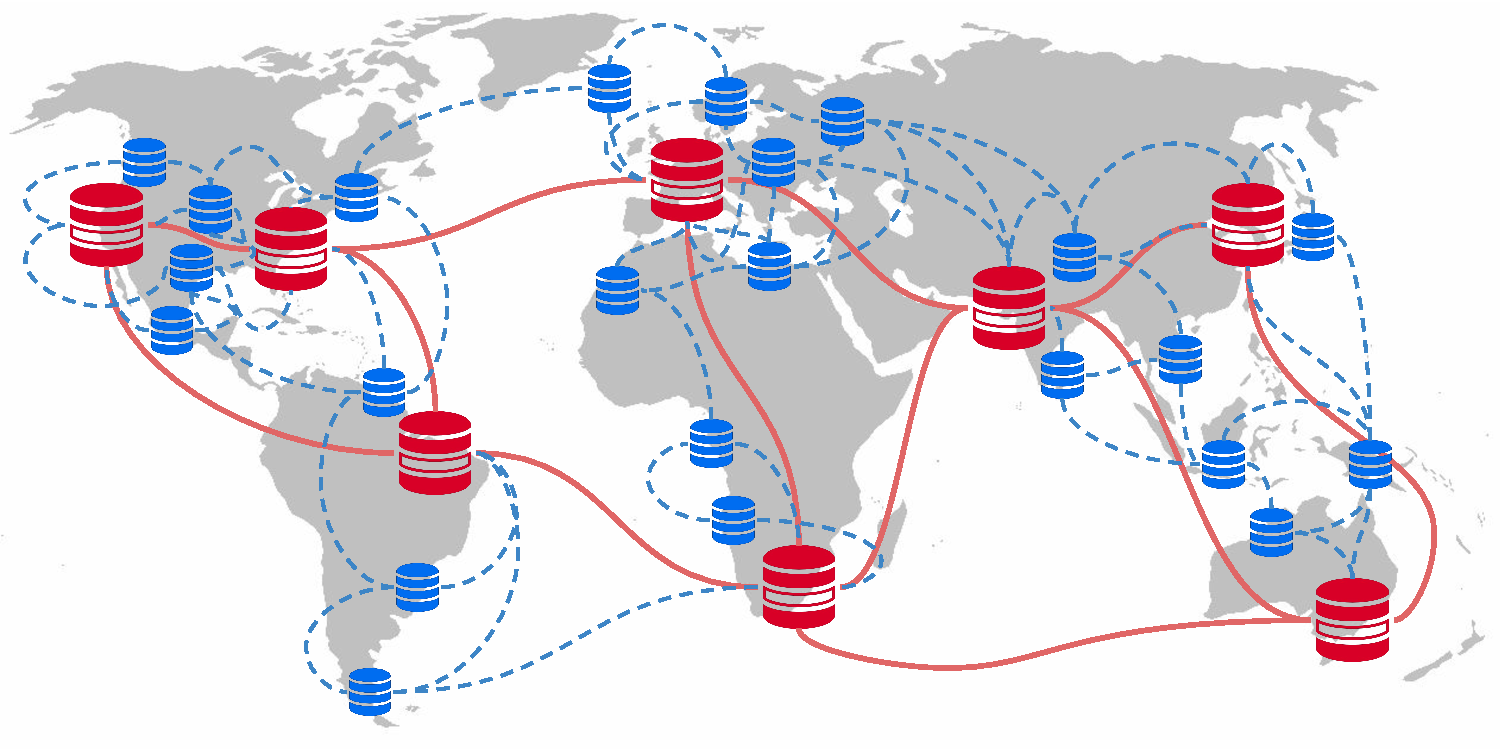
\includegraphics[width=5in]{figures/ch02_global_architecture.pdf}
    \end{center}
    \renewcommand{\baselinestretch}{1}
    \small\normalsize

    \begin{quote}
        \caption[Global Architecture]{A global architecture composed of a core backbone of hierarchical consensus replication (red) and a fog of heterogenous, federated consistency replicas (blue).}
        \label{fig:ch02_global_architecture}
    \end{quote}
\end{figure}
\renewcommand{\baselinestretch}{2}
\small\normalsize

Modern software applications require a strong consistency model that is region-agnostic.
Hierarchical consensus provides that consistency model by unifying coordination into a single-process model rather than having multiple, independent processes all coordinating accesses.
Hierarchical consensus ensures that there is an intersection between namespace coordination and access coordination so that there is a provably strong relationship between the participation of all replicas in consensus across the globe.
This relationship ensures that a general audience of developers can reason about consistency, geolocate data, and deploy systems without the complexity of most systems.

The next generation of systems will also require high-throughput writes from a mobile, heterogenous network.
Rather than relying on the centralizing effect of the cloud, we also propose to augment our system with a decentralized fog of highly available replicas.
These replicas use traditional eventually consistent systems to ensure high-availability for writes at the cost of a high likelihood of stale reads.
We propose that this outer edge layer is not independent of the centralized applications, but rather we propose a federation of consistency models that increases global consistency.
Federated consistency allows replicas to choose at which consistency level they participate in the system, creating a continuous, hybrid consistency across independent objects.

The base application we have constructed is a key/value store as described in Chapter~\ref{ch:system_implementation}.
Keys serve as the basis for sharding in our system and allow us to generically apply dependency relationships depending on the application.
Key/value stores can be seen as the underlying storage for databases, but we target two other applications: a distributed ledger and a file system.
Distributed ledgers have recently grown in popularity thanks to decentralized blockchain protocols~\cite{fruitchains}.
Hierarchical consensus can be used to quickly export a per-object or multi-object distributed log.
Key/value stores can also be used for underlying file systems~\cite{s3}.
Many high-performance distributed databases rely on an underlying replicated file system~\cite{aurora,btrdb,bigtable,megastore,spanner}.
We believe that a planet-scale file system will therefore provide the best platform to construct a myriad of services that are themselves planet-scale.

\section{Conclusion}
\label{ch02_conclusion}

In this chapter we have presented the challenges, motivations, and background of today's geo-replicated data systems.
Modern software systems are now developed with international audiences in mind, largely due to the success of large Internet companies that provide cloud infrastructure around the world.
As the demand for global-scale software has grown, so to has the need for geo-replicated services, however, while cloud providers have provided access to provisioned large scale databases, these database have been specialized and optimized for the applications they were built for, not a general audience.
The result is that software developers have to deeply consider consistency and localization semantics at the application level, which leads to confusion.

The challenge is that the current generation of geo-distributed systems rely on a pristine data-center environment, able to support a multi-process architecture on high-performance machines and networks.
Multi-process architectures have multiple levels of coordination and replication, making it extremely difficult to reason about the consistency model.
Moreover, the next generation of geo-distributed system will not reside in data-centers, but in more variable, mobile network environments.
To accommodate both of these trends, we have proposed a consistency-centric architecture for planet-scale systems.

The primary challenges for a planet-scale systems are their scale and the variability of the connections between participants.
Our architecture places primary importance on durability, fault-tolerance, heterogeneity, and adaptability by specifying two federated tiers of access.
The first tier, inside of data centers, uses hierarchical consensus to provide strong geo-replicated consistency as well as catastrophic failure tolerance by replicating data cross zones and regions.
The second tier, at the edge in the mobile network federates a highly available system model with a strong consistency model to provide stronger global guarantees.
Finally, our system self-organizes by monitoring access patterns and the network environment, adapting to change to provide resilience over time.

In the next chapter, we will explore the core component of this dissertation: hierarchical consensus.
